% !TEX root = ../../main.tex
\section{Results}\label{sec:real_world_results}
In this section we will provide the results of our methods applied to the real-world data sets and discuss the quality of the solution.
As stated above, we will use the objective quality metrics as used in \Cref{sec:artificial_data_quality_metrics}.
That will be in the form of a tabular overview of the (manually set) best meta-parameters and results, expressed in \gls{far} and $\operatorname*{Average\_delay}$ (following \Cref{sec:artificial_data_results}).
Furthermore, we will discuss the results from an empirical point of view, since the problem of finding change points in human activities is ambiguous.
By stating our observations and remarks and providing fragments of visual results, we will discuss the characterizing strengths and weaknesses of our method.

\subsection{Objective metrics}
The employed two-stage algorithm requires the setting of user defined parameters.
In \Cref{tab:results_real_world} for each run the results are listed, together with the used parameters.
We have used a window length of 50 frames, which represents around $1.16$ seconds of data (the frame-rate of the recordings is not fixed).
The other parameter values, \ie the \gls{rbf} $\sigma$, high and low threshold and closeness factor, are the result of an educated guess and manual optimization.
In general, a high value for the upper threshold and low value for the lower threshold indicates a robust method, since it indicates that change points are significantly different from homogeneous segments.
The closeness time frame should be low, since that indicates there are few false positives.

\begin{table}
  \centering
  \caption[Results real world runs]{Parameter settings and results of the real-world data sets.}
  \begin{tabulary}{\textwidth}{|l|c|c|c|c|c|c|c|}
    \cline{2-8}
    \multicolumn{1}{l|}{} & Run 1 & Run 2 & Run 3 & Run 4 & Run 5 & Run 6 & Run 7 \\
    \hline
    Window length & 50 & 50 & 50 & 50 & 50 & 50 & 50 \\
    \hline
    Sigma of \gls{rbf} & 13 & 13 & 13 & 13 & 13 & 13 & 4 \\
    \hline
    High threshold & 1.2 & 1.5 & 1.3 & 1.1 & 1.3 & 1.2 & 1.7 \\
    \hline
    Low threshold & 0.8 & 0.8 & 0.6 & 0.7 & 0.7 & 0.8 & 0.6 \\
    \hline
    Closeness (s) & 0.7 & 0.85 & 1 & 0.6 & 0.7 & 1 & 0.8 \\
    \hline
    \hline
    $\operatorname*{far}(Y)$ & 0.1 & 0.05 & 0 & 0 & 0.2 & 0 & 0.48 \\
    \hline
    $\operatorname*{Average\_delay}$ & 0.52 & 0.83 & 0.47 & 0.92 & 1.26 & 1.05 & 0.92 \\
    \hline
    STD Delay & 0.29 & 0.55 & 0.52 & 0.75 & 1.67 & 0.78 & 0.92 \\
    \hline
  \end{tabulary}
  \label{tab:results_real_world}
\end{table}

To give a better impression on the quality of the $\operatorname*{Average\_delay}$, \Cref{fig:boxplot_real_world_runs} shows a box plot for each run.
It shows the spread of the $\operatorname*{Average\_delay}$ in seconds over all the change points.
A lower and more compact box plot is better.

\begin{figure}
\centering
  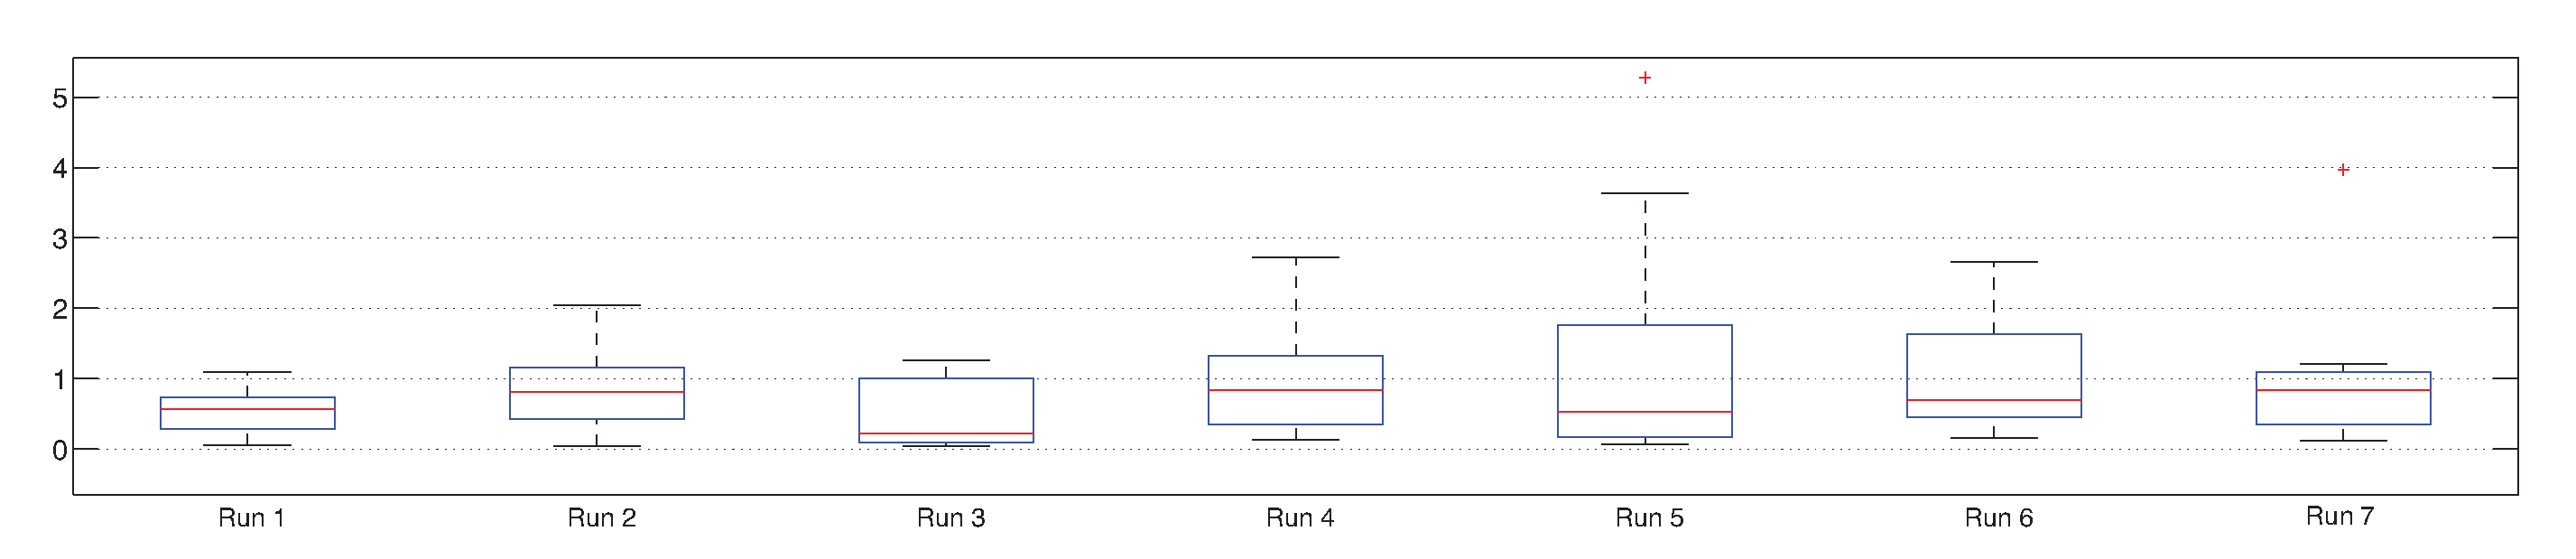
\includegraphics[width=1\textwidth]{./Figures/chapter6/data_collection/boxplot_results_real_world_runs.eps}
  \caption[Box plot results real-world runs]{Box plot of the results for the real-world runs, indicating the number of data points between the actual and closest detected change points. A lower and more compact box plot is better.}
  \label{fig:boxplot_real_world_runs}
\end{figure}

\subsection{Subjective observations and remarks}
It can be ambiguous where to place the (manually annotated) change points, in the case of real world data.
The objective quality measure can give a distorted view on the performance.
To overcome this, we will state observations and remarks found after close (visual) inspection of the annotated and discovered change points.
In \Cref{fig:plots_all_runs_results} all the results are plotted.
The black solid lines indicate our manually determined change points.
The dashed purple lines indicate the change points as discovered by our method.
We will start with general observations applicable to all the runs and will continue with individual remarks for each run.
Where possible, a graphical illustration will support our observations.

Overall our impression is that the proposed method is fairly good at recognizing change points.
Depending on the parameters for the sensitivity adjustment, almost all changes are discovered.
With a high sensitivity it seems, initially, the method produces many false positives.
After closer inspecting of the data, we can confirm that there is a change in the data, although the performed activity stayed the same.
This is also a weakness of the method: since the sensitivity is set globally, it can produce many semi-false positive change points for some segments of a run.

An other positive observation is that the method often recognizes a change point \emph{before} our annotation.
Again, after closer inspection we can see that the data changes shape and distribution before we annotated a change based on the video recordings.
This effect can be observed in the case of a transition from running to walking; the last `steps' of running are already recognized of being different.
As with the above behavior, this is subject to parameter settings.

Considering the overall performance and results, we have the following observations of cases in which the method has problems with detecting change:
\begin{itemize}
  \item \textbf{Merging:} in our method we use a \emph{closeness} time period $t_c$ (usually up to $0.5$ - $1.0$ seconds) to merge discovered change points that have a very small distance between them.
  Multiple merging-strategies can be applied, and in our method we use the naive implementation by simply ignoring all the discovered change points that occur less than $t_c$ seconds after the previous change point.
  This works well when there is a block of noisy data with a high amount of (falsely) discovered change points.
  On the flip side, this method will ignore real new change points which occur during the noisy period.
  This problem on itself can be formulated as a change detection problem.
  \item \textbf{Masking:} Since the parameters for the detection method are set globally, it is difficult to discover all the change points (and only the change points) without a high \gls{far}.
  If a change point is proceeded by a noisy block, then the real change point will be merged with the previous change points.
  In an other case, where a change point is very clear represented in the data but the next, close by, other change point is more subtle, the latter change point is \emph{masked} by the former.
  This masking effect is also discussed in \cite{inclan1994use}, where an iterated approach is applied.
  \item \textbf{False heterogeneity:} For our video-data synchronization, we started and ended each recording with a few seconds in which the recording smartphone was kept still in the air.
  During this period, the data variance, and thus the constructed hypersphere, becomes very small.
  As a results, even small movements are considered to be changes and in the case of the mid-air still smartphone a lot of false change points are detected.
  Due to the merging effect described above, the final real change point (often shaking the smartphone) is not discovered.
  \item \textbf{Incorrect weighting:} In our analyses we have used the data from the accelerometer, magnetic field, and rotation sensors.
  In the segments which embodied movement in a circular manner (such as walking and running around a fountain), the turn was not (or at a different time point) discovered.
  Alternatively, when we only used the magnetic field and rotation sensors, the turn was correctly discovered.
  Other transitions, such as from walking to running, are harder to discover without the (linear) accelerometer sensor data.
\end{itemize}

When looking at the individual runs, we have the following observations for each run number:
\begin{enumerate}
  \item \textbf{Subject 2, straight walk and run} \Cref{fig:data_with_cps_run_1}
    \begin{itemize}
      \item The first transition from running to walking, around $14s$ is harder to discover than the transition for the same activities around $33s$.
      This shows is that in real-world applications there is a diversity between the same transitions and activities.
      \item Around $8s$, $9s$, and $16s$ a few steps (while walking) are regarded as change points.
      During the running segments from $17s$ and $28s$ there is a lower probability of change for each step.
    \end{itemize}
  \item \textbf{Subject 1, straight walk and run} \Cref{fig:data_with_cps_run_2}
    \begin{itemize}
      \item Following the video recordings, we have annotated a change point from running to walking around $37s$.
      Our method discovers a change point almost a second before.
      In retrospect, we can see that the data distribution indeed changes from the discovered change point on.
      This shows us two important principles.
      The first is that the annotations are very subjective.
      The second is that between different activities the transition period is longer than we would think.
      Looking at the data, we can see that the body slows down, even before we visually notice it on the video recordings.
    \end{itemize}
  \item \textbf{Subject 2, walk around corner} \Cref{fig:data_with_cps_run_3}
    \begin{itemize}
      \item The $90^{\circ}$ counter-clockwise turn during the walking activity is hard to discover when the accelerometer sensor data is included.
      When only the magnetic field and rotation sensors are used, the turn requires a lower sensitivity.
      With only these two sensors all the other change points in this run are also successfully discovered.
    \end{itemize}
  \item \textbf{Subject 2, walk and run around fountain} \Cref{fig:data_with_cps_run_4}
    \begin{itemize}
      \item Like in the first run, the walking segment from $24s$ results in a change point for each step.
      Further inspection of the data reveals that each step is indeed different from the other.
      Due to the global parameter settings, the sensitivity is too high for this segment to recognize it as one.
      It could also be that our used window-length is too small, to model a good representation of this segment.
      \item During the circular run, from $12s$ till $24$, there are two change points discovered.
      The difference for the rotational vectors need to accumulate to a certain value before they have enough influence to let the rotation be regarded as a change point.

    \end{itemize}
  \item \textbf{Subject 1, walk and run around fountain} \Cref{fig:data_with_cps_run_5}
    \begin{itemize}
      \item As with the other runs, the accelerometer data makes it harder to detect turns.
      It requires a higher sensitivity, which results in a higher \gls{far}.
    \end{itemize}
  \item \textbf{Subject 2, walk and run fountain 2} \Cref{fig:data_with_cps_run_6}
    \begin{itemize}
      \item During the standing segment around $38s$ there are a lot of false positives.
      It seems to be the \emph{false heterogeneity} problem described above.
    \end{itemize}
  \item \textbf{Subject 3, indoor stairs} \Cref{fig:data_with_cps_run_7}
    \begin{itemize}
      \item The walking segment around $22s$, between two segments of walking downstairs, shows little difference in the data.
      To recognize it as a change point a high sensitivity and low closeness time period $t_c$ is required.
      \item During some segments (downstairs from $24s$, upstairs from $42s$ and $54s$) the method discovers more change points than our annotation.
      A closer inspecting of the raw data reveals indeed changes in behavior.
      To exclude these (semi) false positives, a better tuning of parameters is required.
      \item Because of the circular shape of the stairs, the magnetic field sensors constantly differs.
      Although our method is build to exclude slow shifting changes (because we are only interested in sudden changes), with our used window width it still eventually results in change points.
      \item The difference between taking the stairs and walking is smaller than, \eg, walking and running.
      The delay between these segments seems to be larger, as illustrated around $33s$.
    \end{itemize}
\end{enumerate}

\begin{figure}
  \centering
  \begin{subfigure}{1\textwidth}
    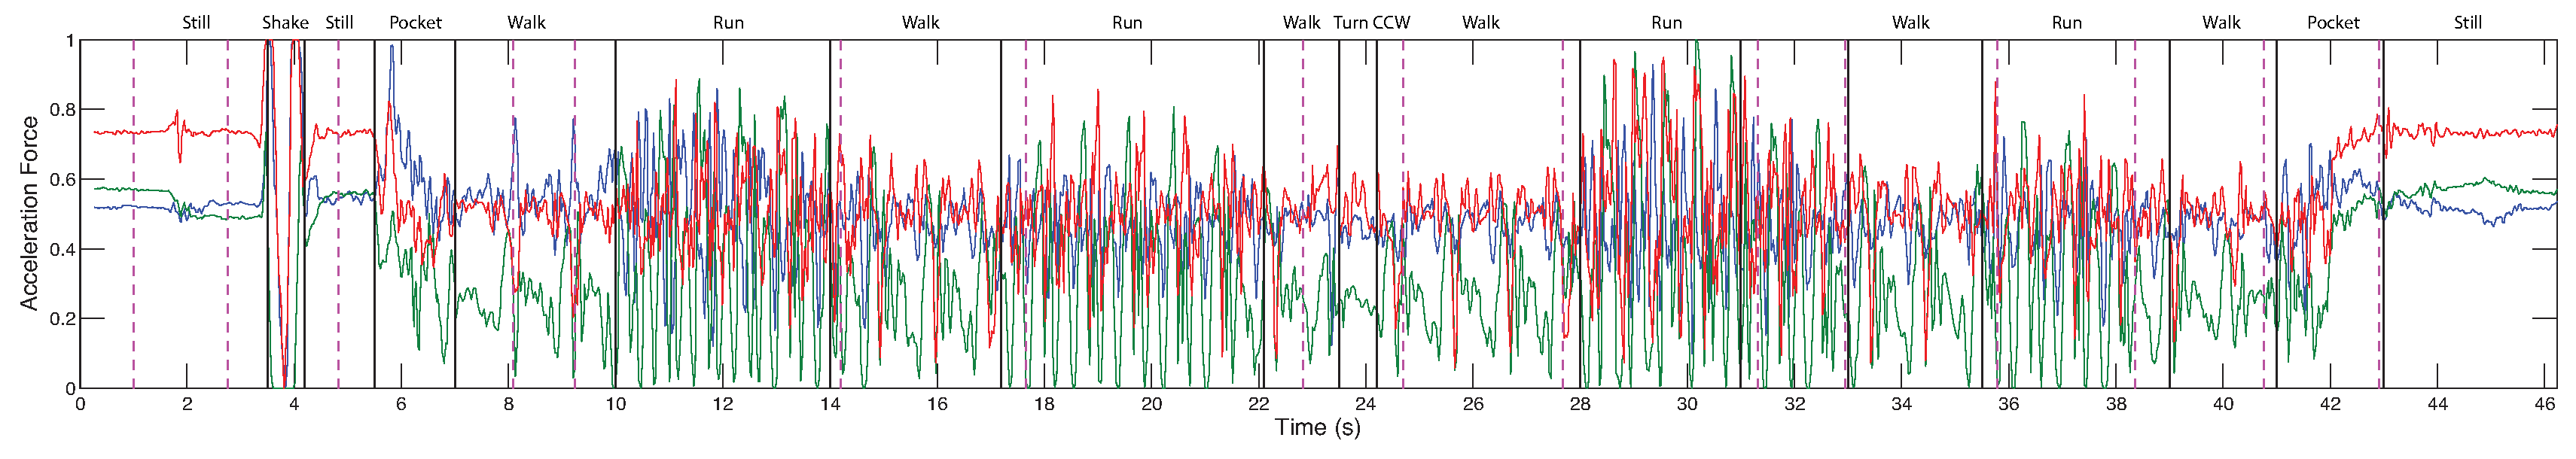
\includegraphics[width=\textwidth]{./Figures/chapter6/data_collection/run-1-walk-run-roemer/data_plot_acc_with_discovered_cps.eps}
    \caption{Run 1}
    \label{fig:data_with_cps_run_1}
  \end{subfigure}

  \begin{subfigure}{1\textwidth}
    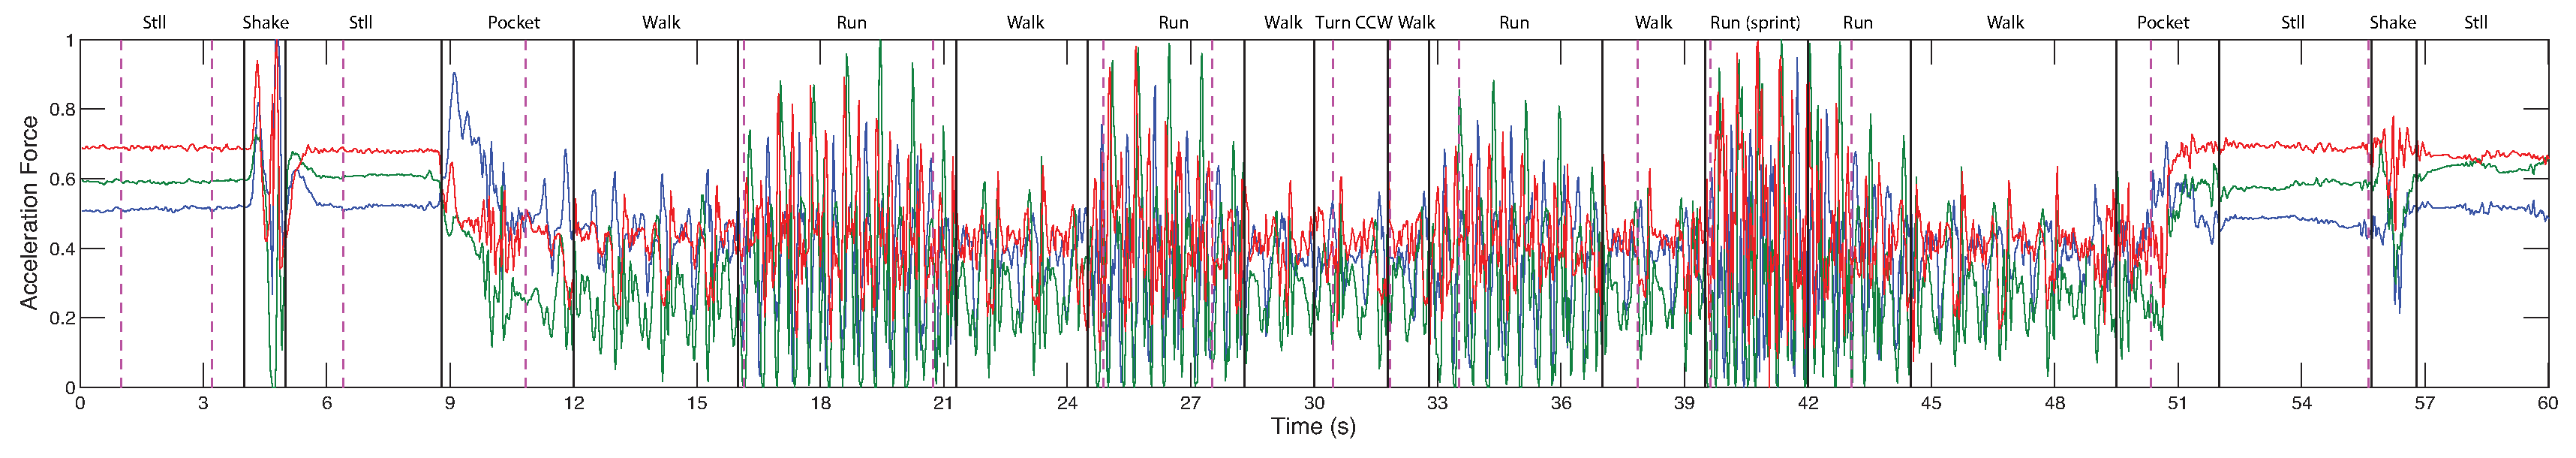
\includegraphics[width=\textwidth]{./Figures/chapter6/data_collection/run-2-walk-run-jos/data_plot_acc_with_discovered_cps.eps}
    \caption{Run 2}
    \label{fig:data_with_cps_run_2}
  \end{subfigure}

  \begin{subfigure}{1\textwidth}
    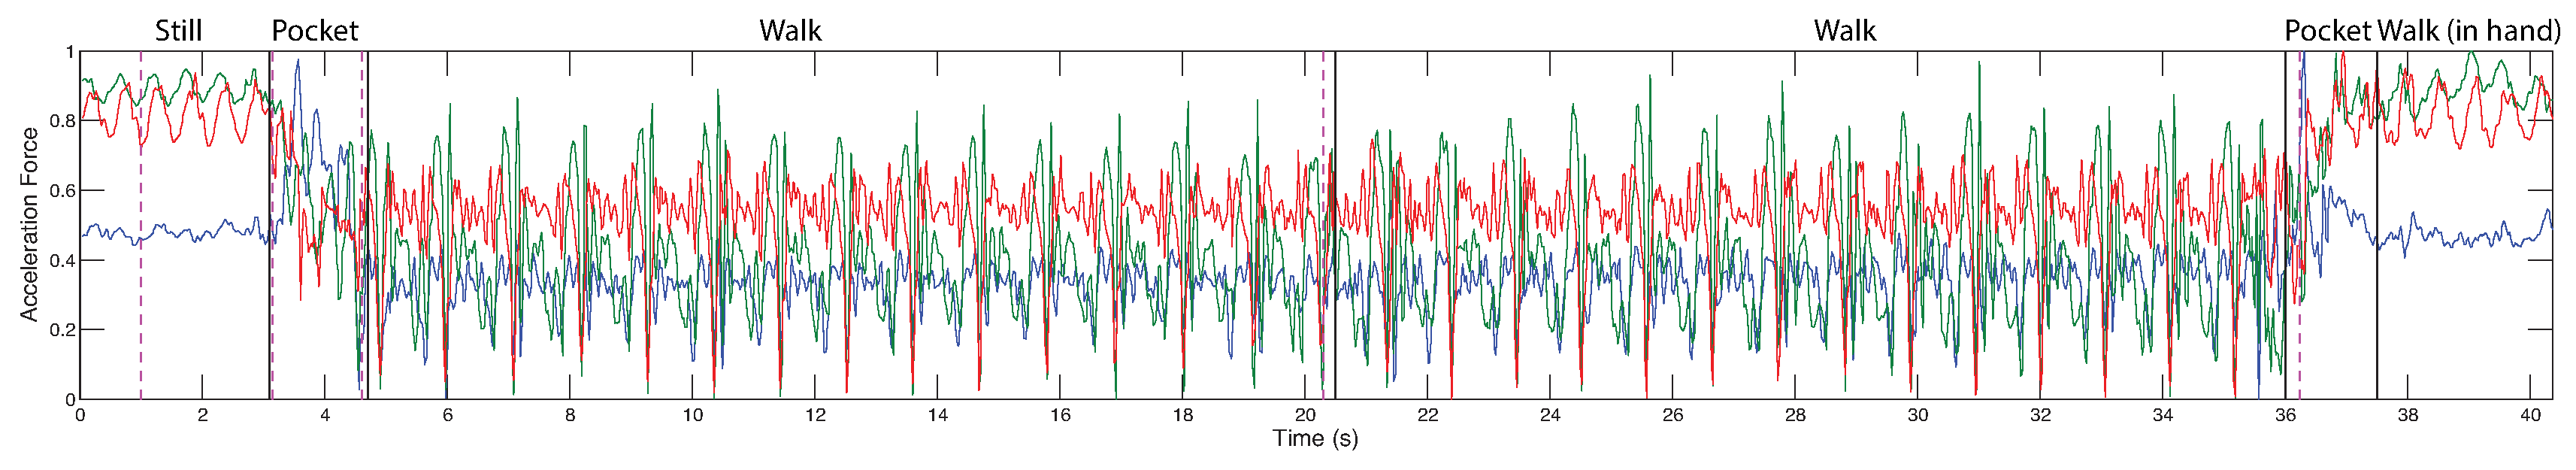
\includegraphics[width=\textwidth]{./Figures/chapter6/data_collection/run-3-walk-turn-roemer/data_plot_acc_with_discovered_cps.eps}
    \caption{Run 3}
    \label{fig:data_with_cps_run_3}
  \end{subfigure}

  \begin{subfigure}{1\textwidth}
    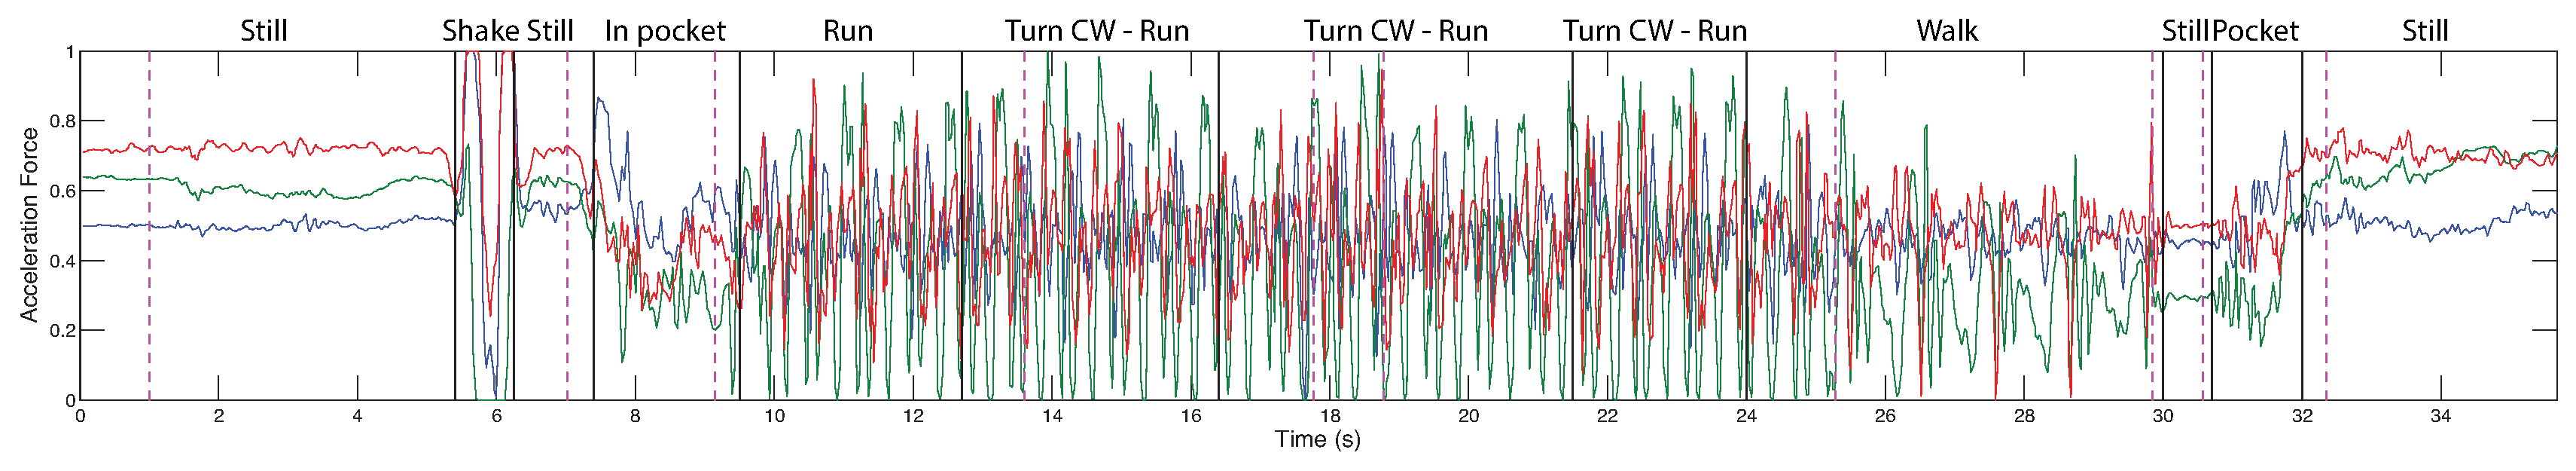
\includegraphics[width=\textwidth]{./Figures/chapter6/data_collection/run-4-run-fountain-roemer/data_plot_acc_with_discovered_cps.eps}
    \caption{Run 4}
    \label{fig:data_with_cps_run_4}
  \end{subfigure}

  \begin{subfigure}{1\textwidth}
    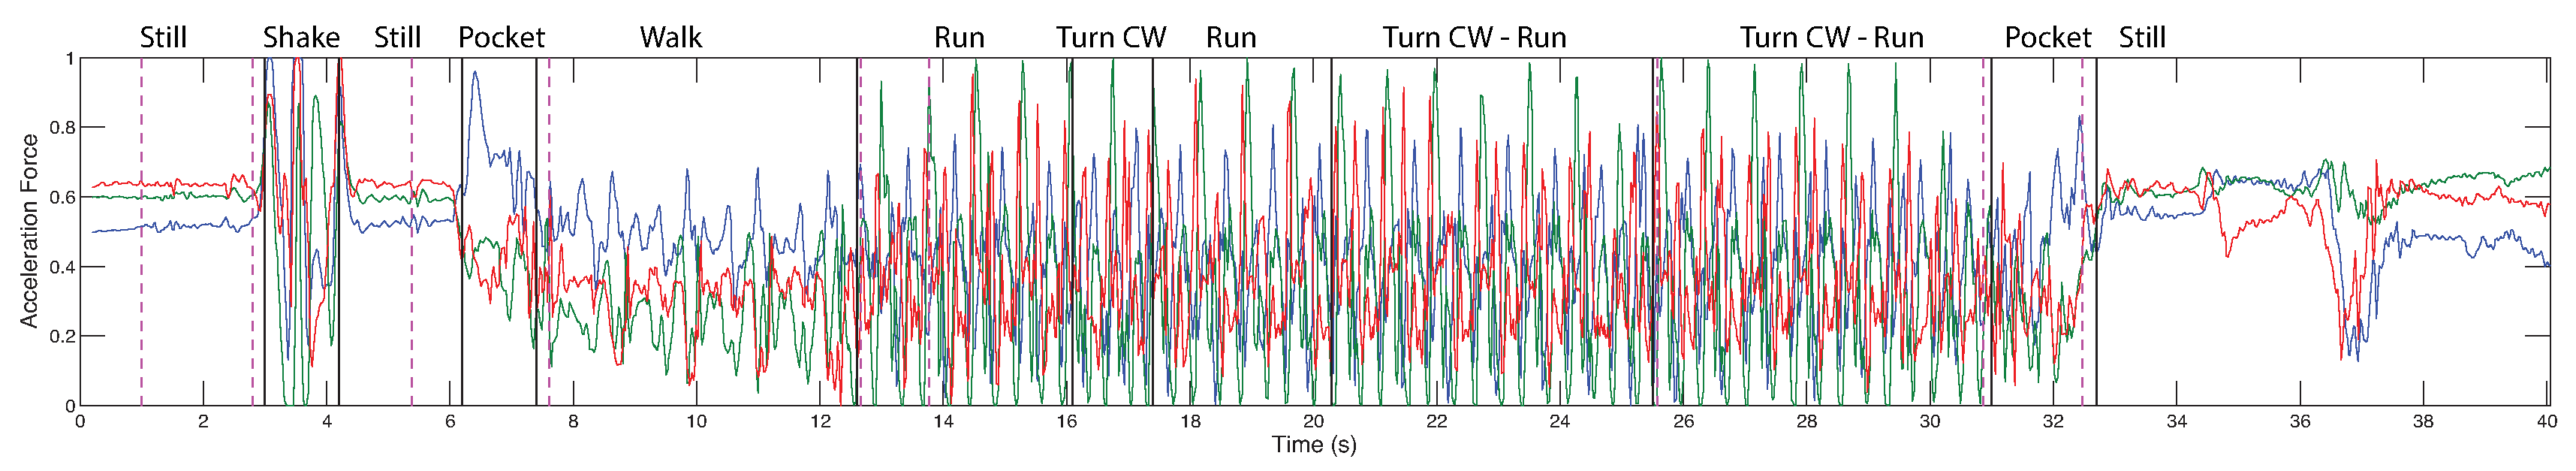
\includegraphics[width=\textwidth]{./Figures/chapter6/data_collection/run-5-run-fountain-jos/data_plot_acc_with_discovered_cps.eps}
    \caption{Run 5}
    \label{fig:data_with_cps_run_5}
  \end{subfigure}

  \begin{subfigure}{1\textwidth}
    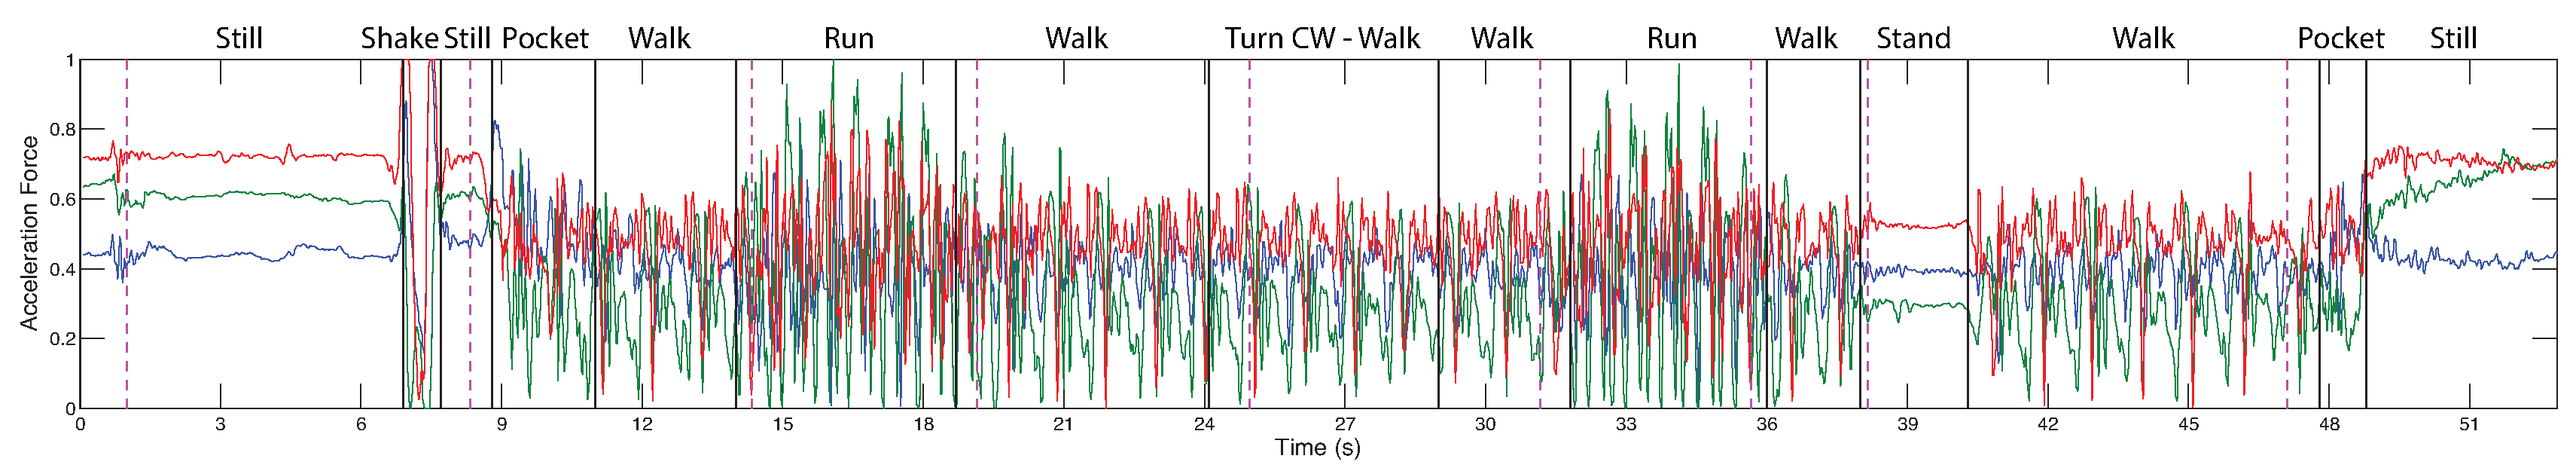
\includegraphics[width=\textwidth]{./Figures/chapter6/data_collection/run-6-walk-run-roemer/data_plot_acc_with_discovered_cps.eps}
    \caption{Run 6}
    \label{fig:data_with_cps_run_6}
  \end{subfigure}

  \begin{subfigure}{1\textwidth}
    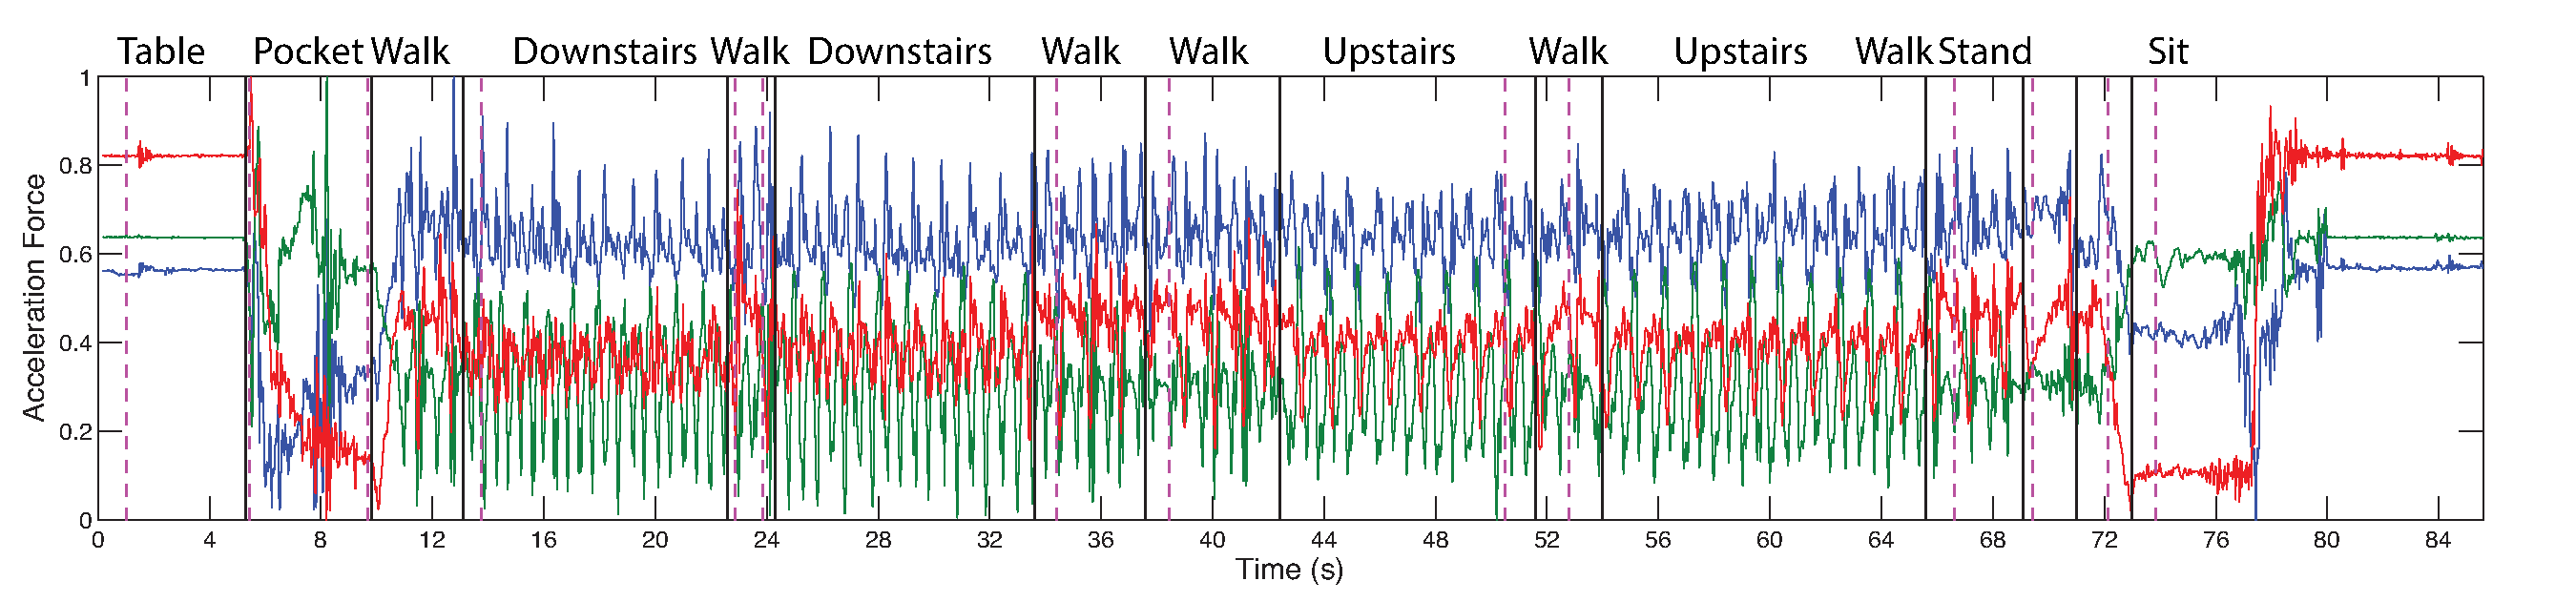
\includegraphics[width=\textwidth]{./Figures/chapter6/data_collection/stairs-1-marc/data_plot_acc_with_discovered_cps.eps}
    \caption{Run 7}
    \label{fig:data_with_cps_run_7}
  \end{subfigure}

  \caption[Results run 1/8]{Annotated plots of all runs. The black vertical lines are manually determined change points, the purple dashes lines are the discovered change points. The label above each segment indicates the current performed activity.}\label{fig:plots_all_runs_results}
\end{figure}


\section{Possible improvements}\label{sec:possible_improvements}
From the above section we can extract a few possible improvements for the algorithm.
Most of the observations and remarks are due to a different required sensitivity for local segments of the run.
Currently, our method employs a global setting for the thresholds.
A possible improvement would be to use locally optimized parameters, although that would require an reflective data processing approach or more a priori information about the data.
With our approach, the lack of a priori knowledge about the data distribution is one of the design decisions.

Furthermore, we discovered that sometimes, especially with movements incorporating circular motions, the addition of (linear) accelerometer data makes the discovery of change points harder.
In such cases, each of the inertial sensor data streams should be relatively weighted (\eg using the covariance) in order to signal an overall change when it only occurs in one of the streams.